%%=============================================================================
%% Methodologie
%%=============================================================================

\chapter{\IfLanguageName{dutch}{Methodologie}{Methodology}}
\label{ch:methodologie}

%% TODO: Hoe ben je te werk gegaan? Verdeel je onderzoek in grote fasen, en
%% licht in elke fase toe welke stappen je gevolgd hebt. Verantwoord waarom je
%% op deze manier te werk gegaan bent. Je moet kunnen aantonen dat je de best
%% mogelijke manier toegepast hebt om een antwoord te vinden op de
%% onderzoeksvraag.

In dit hoofdstuk gebeurt het effectieve onderzoek. Hier zal men starten  met de algemene vergelijking van de gekozen content management systemen, men zal op basis van volgende factoren: intuïtiviteit, customization, support, community, onderhoudbaarheid, governance, performance, integratie en SEO. Op basis van deze vergelijking zullen we de eerste onderzoeksvraag beantwoorden. Daarna wordt er gefocust op het e-commerce aspect van dit onderzoek. In dit aspect gaat men enkele e-commerce extensies met elkaar vergelijken. Deze vergelijking zal gebeuren op basis van volgende factoren: intuïtiviteit, support, all-in-one functionaliteit, governance en SEO. Aan de hand van deze vergelijking zal men een antwoord formuleren op de tweede onderzoeksvraag.  

\section{De algemene vergelijking tussen Wordpress, Joomla en Drupal }
\subsection{De intuïtiviteit van de backoffice}

\subsubsection{Wordpress}
Wanneer men inlogt komt men in de backoffice van een Wordpress installatie terecht. Hier vindt men een dashboard met verschillende widgets terecht. Deze zijn makkelijk te expanden, collapsen en te herschikken. Er kan makkelijk ingesteld worden welke men wenst weer te geven en welke niet. Standaard zijn er 5 widgets geïnstalleerd. Men kan nieuwe widgets toevoegen door te coderen. Deze widgets verhogen de user experience van de backoffice.

Zoals je in figuur 3.1 kan zien, vindt men een menu met de belangrijkste administratieve functionaliteiten. Er wordt een splitsing gemaakt tussen content functionaliteiten en de meer technische en design gerichte functionaliteiten. Bij een standaard installatie van Wordpress is dit onderscheid duidelijk zichtbaar maar, naarmate er extra functionaliteit wordt toegevoegd wordt dit onderscheid minder overzichtelijker. 

De backoffice biedt een groot assortiment van talen aan, er kan makkelijke veranderd worden tussen talen. Meestal is er één default taal ingesteld die door de meeste gebruikt worden, maar er is ook de mogelijkheid om per gebruiker een specifieke taal in te stellen. Dit laatste is een belangrijke gegeven om de user experience van de gebruiker te optimaliseren. In het algemeen voelt de backoffice vrij natuurlijk aan, na even te experimenteren met verschillende functionaliteiten raakt men vlug vertrouwd met de omgeving. De welcome widget helpt de personen die niet goed weten waar starten. 
\begin{figure}
    \centering
    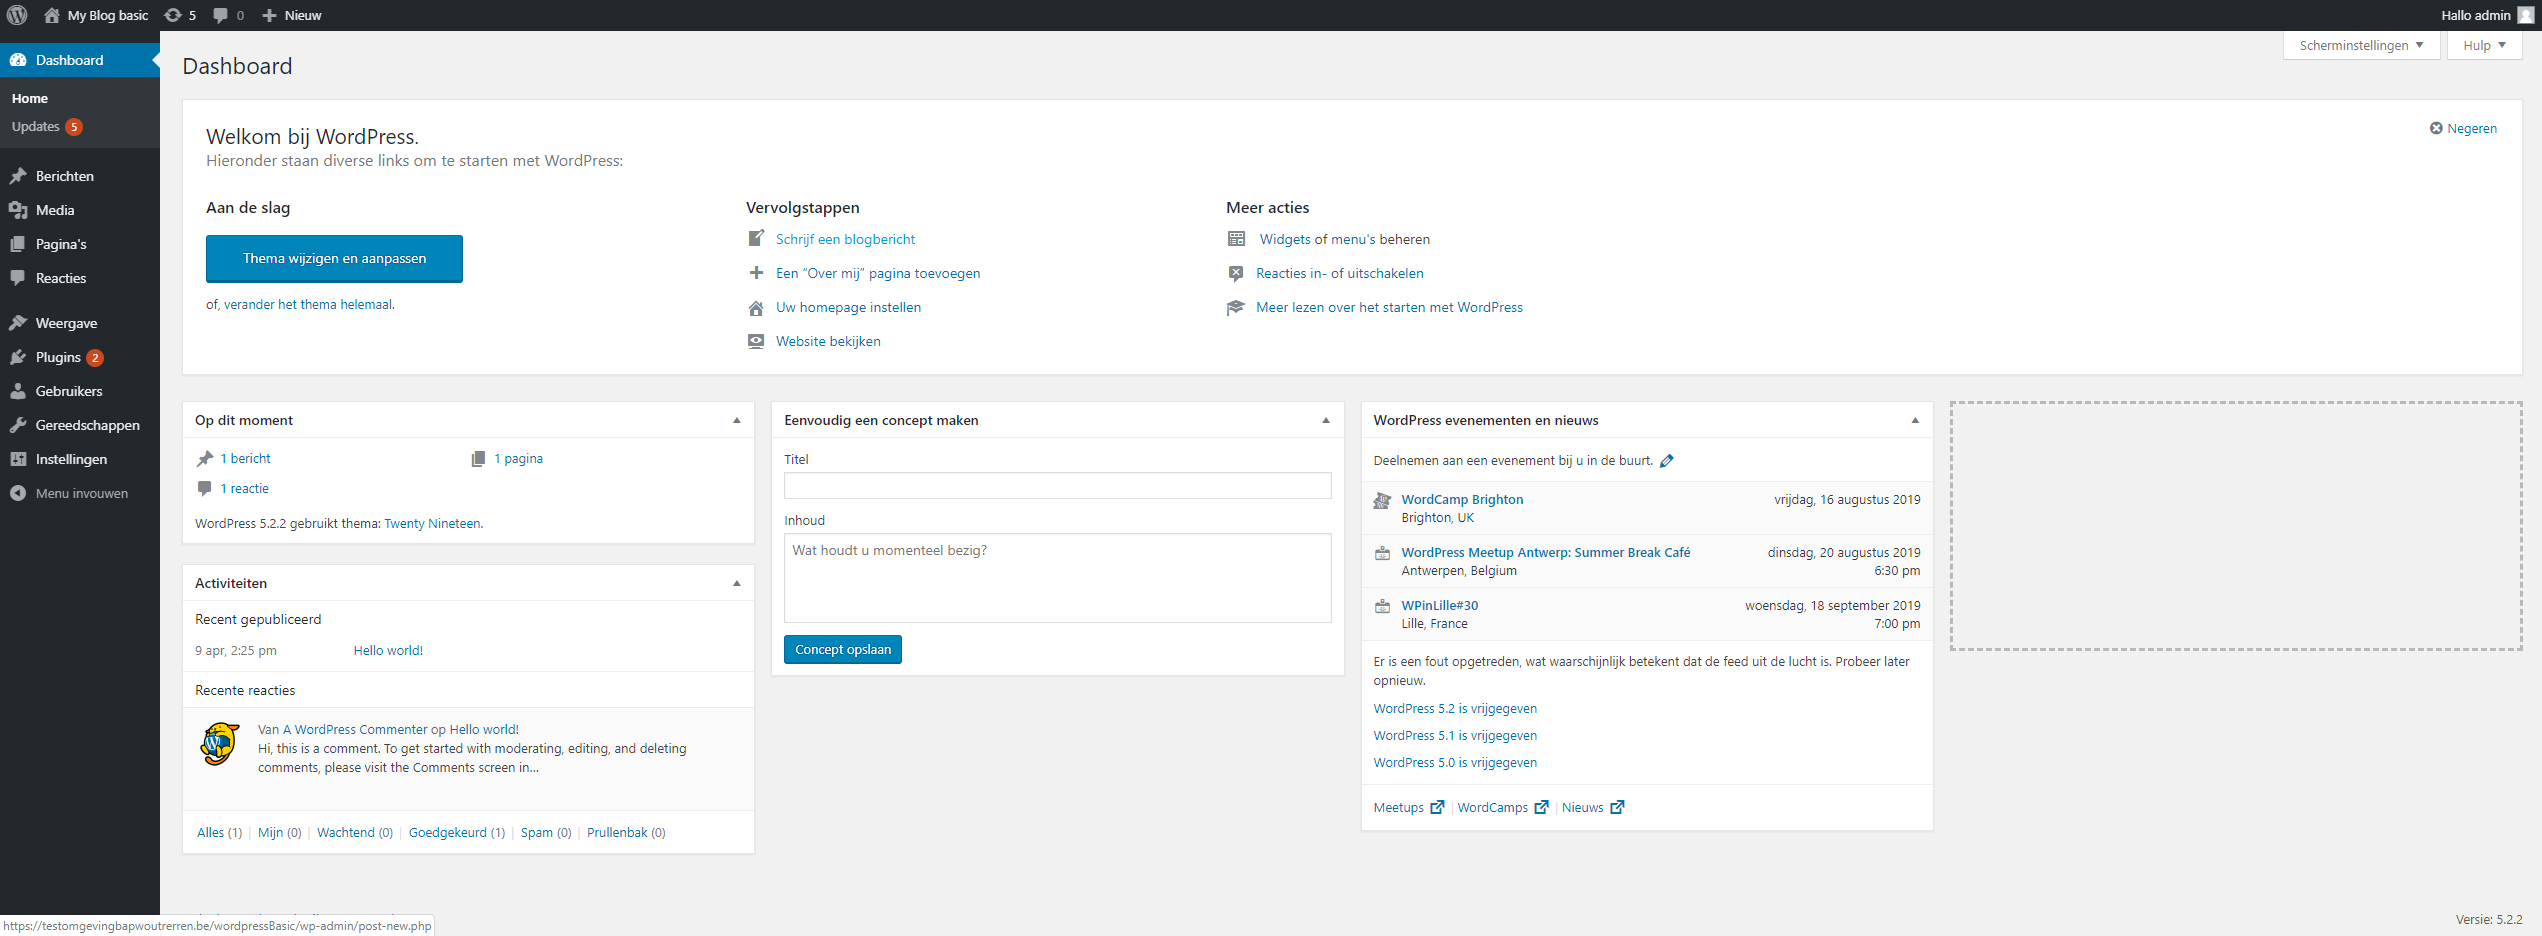
\includegraphics[scale = 0.2]{img/Backoffice_WordPpress.png}
    \caption{De backoffice van een WordPress installatie}
    \label{fig:backofficeWP}
\end{figure}
\subsubsection{Joomla}
Bij Joomla heeft men ook een backoffice. In Joomla heeft deze de naam Control panel gekregen. In figuur 3.2 is het vrij duidelijk dat de lay-out van de backoffice van Wordpress en Joomla  toch enkele gelijkenissen heeft. Bij de control panel is er ook weer een soort dashboard aanwezig met enkele belangrijke gegevens over de website. Links vindt men ook een menu terug met de administratieve functionaliteiten, duidelijk onderscheiden door middel van titels. Deze titels helpen het overzicht bewaren zelfs wanneer er meer menu items bijkomen.

Het control panel is overzichtelijker dan het dashboard van Wordpress, maar het aanpassen ervan voelt minder natuurlijk aan. Bij Wordpress kan men makkelijk de widgets herschikken, collapsen en onzichtbaar maken. Echter bij Joomla moeten men al veel verder gaan zoeken en moeten men meerdere clicks uitvoeren waardoor het hele proces onnatuurlijker gaat aanvoelen. De user experience van de backoffice wordt erdoor negatief beïnvloedt. Hier wordt er ook meerdere talen aangeboden dat we ook per gebruiker kunnen instellen. Echter moet men ook hier weer meer clicks uitvoeren waardoor de algemene user experience achteruit gaat. In het algemeen kan men stellen dat het dashboard aangenaam is en helpvol is bij het op weg zetten voor als men niet goed weet waar starten. Al beïnvloedt de grotere hoeveelheid clicks dat nodig zijn de algemene user experience.

\begin{figure}
    \centering
    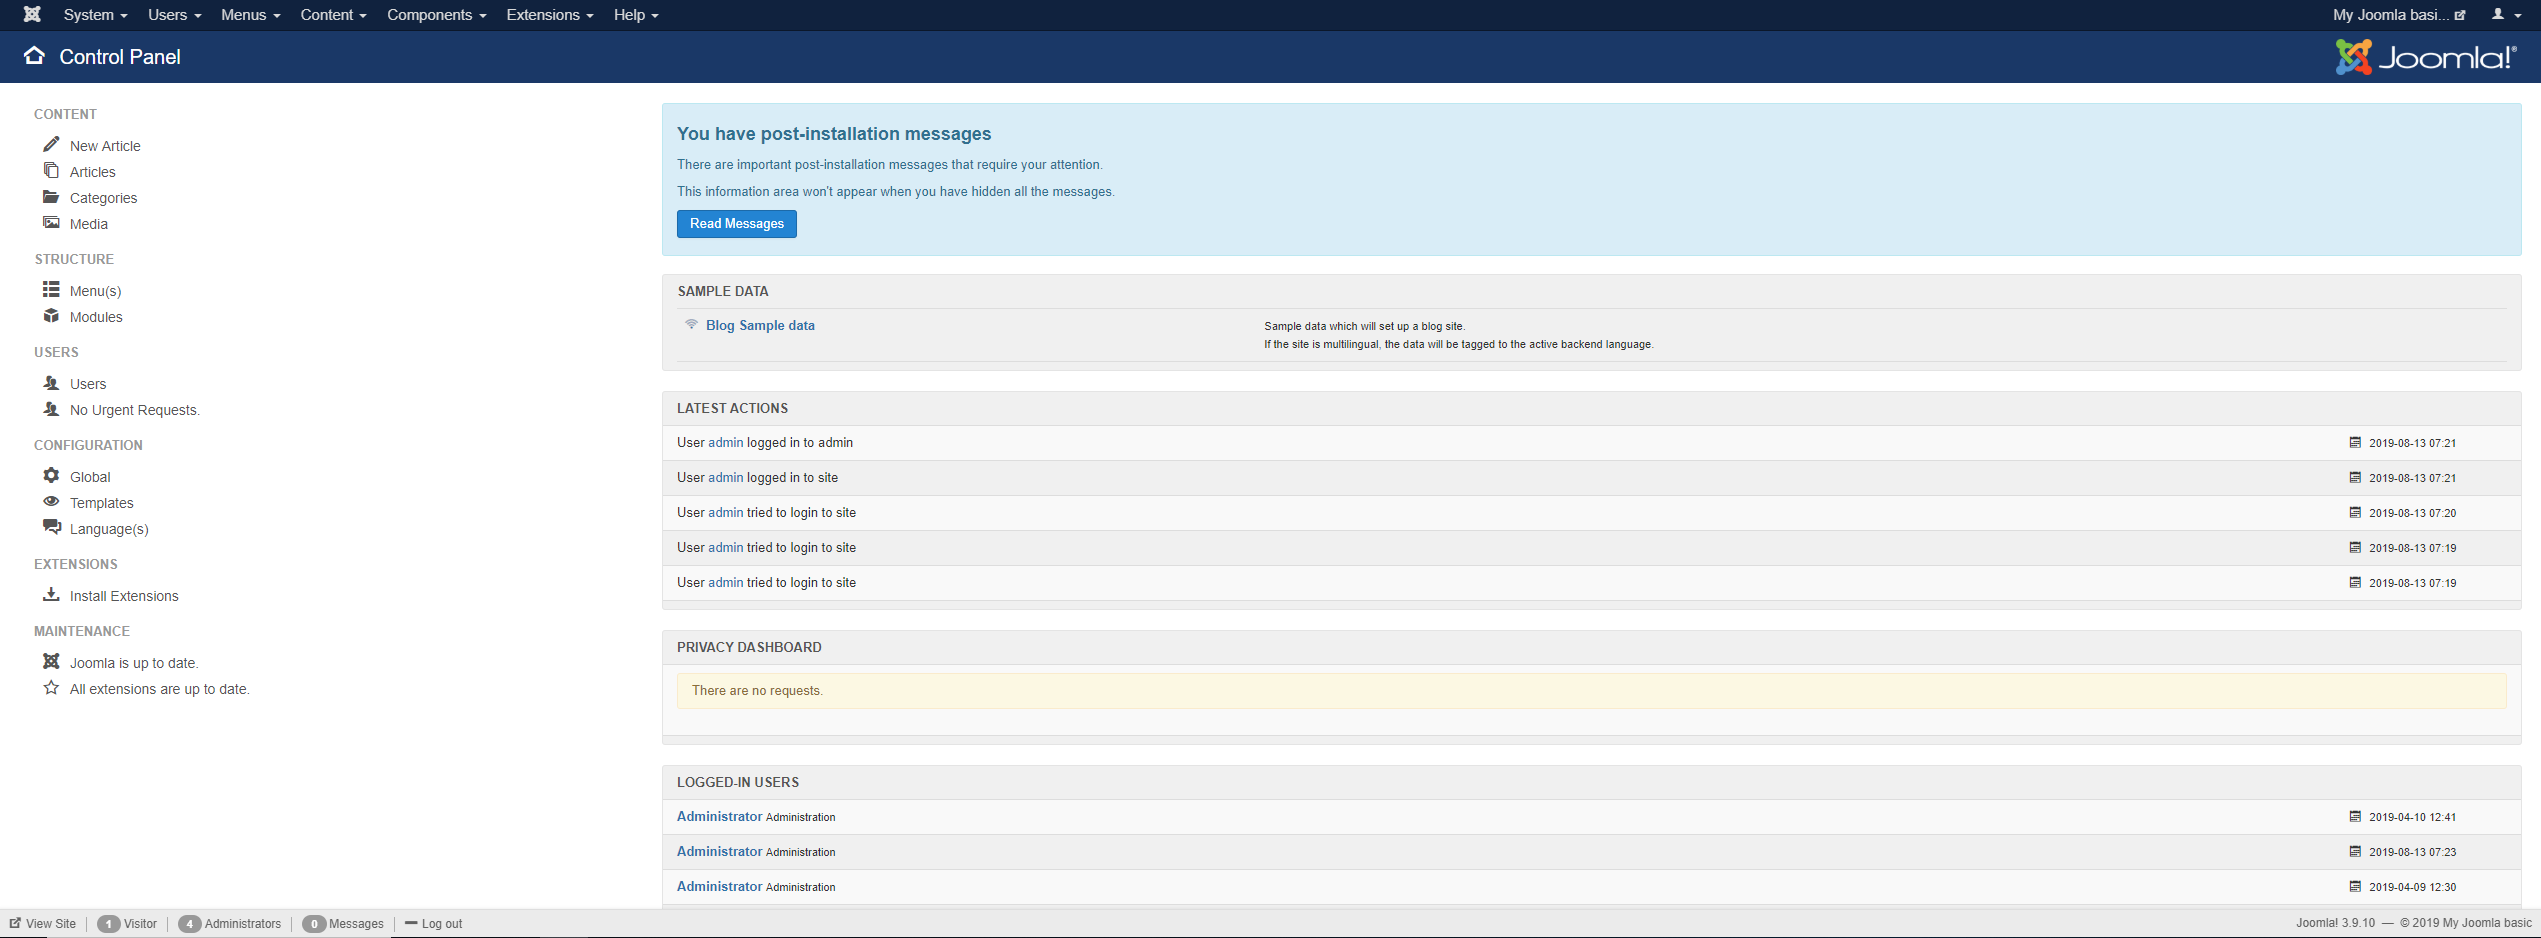
\includegraphics[scale = 0.2]{img/Joomla_controlPanel.png}
    \caption{Control panel van een Joomla installatie}
    \label{fig:controlPanelJoomla}
\end{figure}
\subsubsection{Drupal}
Bij Drupal spreekt men over het adminstratieve menu. Zoals uit figuur 3.3 blijkt is `de backoffice' van Drupal helemaal anders dan die van Joomla of Wordpress. Er is geen dashboard aanwezig. Het menu dat nu horizontaal aanwezig is bevat alle belangrijkste administratieve groepen. Afhankelijk van de modules dat geïnstalleerd zijn en de permissies van de gebruiker kan dit menu verschillen. Op de afbeelding zien we het menu van een nieuwe Drupal 8 installatie als User 1. Men kan deze horizontale menu ook verticaal zetten, de menu neemt dan een interactieve boomweergave aan.

Het voelt minder natuurlijk aan dan bij Joomla en Wordpress, daar werd men via het dashboard op weg gezet naar de eerste stappen dat men kon ondernemen. Bij Drupal voelt het al meer aan dat men duidelijk moet weten waar men naar toe wilt en waar men iets kan terugvinden terwijl dit bij Joomla of Drupal minder het geval is. Men kan wel snelkoppeling definiëren met de belangrijkste administratieve functionaliteiten per gebruiker. Dit verhoogt dan weer de user experience.

Wordpress en Joomla kon men bijvoorbeeld ook makkelijk aanpassen in de gewenste taal en per gebruiker instellen. Drupal moet men al een extra module gaan activeren om de interface te gaan vertalen. Na deze geïnstalleerd is kan men dit perfect vertalen en ook instellen per gebruiker. Dit zijn natuurlijk al een heleboel clicks, waardoor de user experience negatief beïnvloedt wordt. Eenmaal men gewend geraakt is aan Drupal zal men er vlot mee kunnen werken, maar bij het eerste gebruik zal dit niet het geval zijn.

\begin{figure}
    \centering
    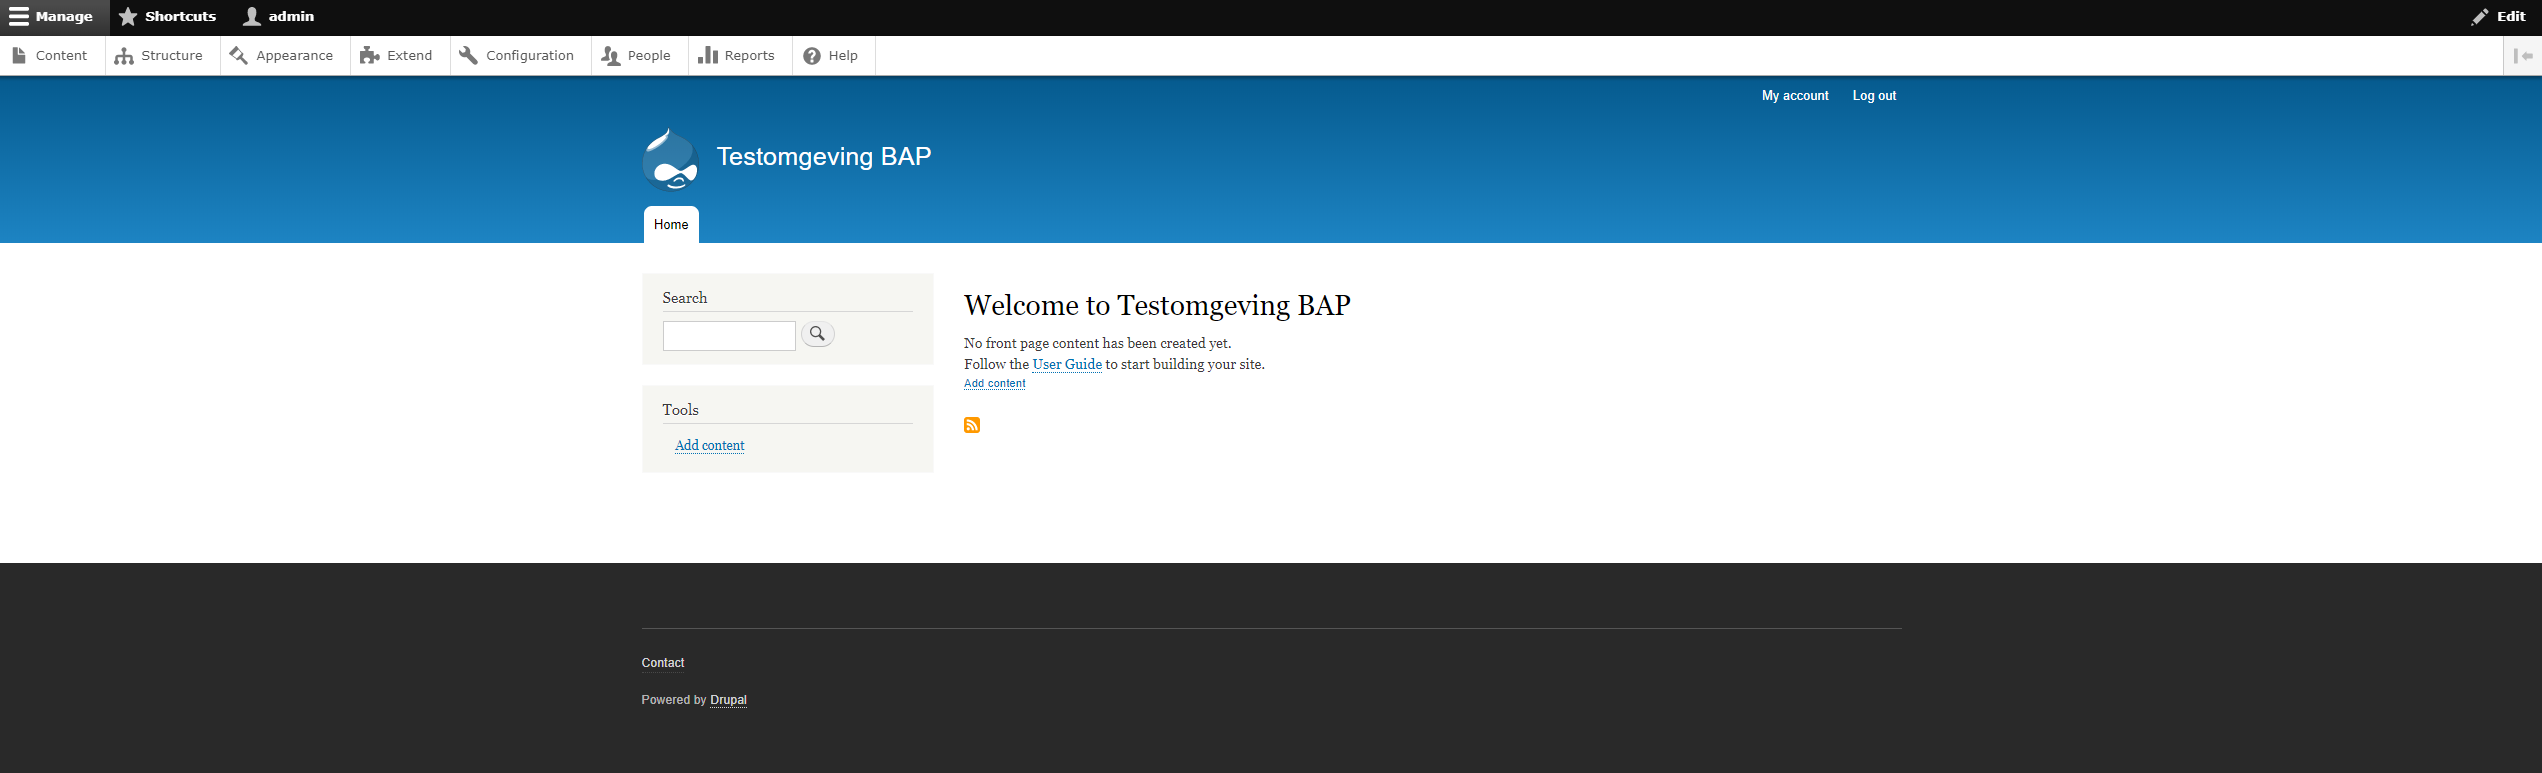
\includegraphics[scale = 0.2]{img/Drupal_Admin.png}
    \caption{Administratieve menu van een Drupal installatie}
    \label{fig:adminDrupal}
\end{figure}

\subsection{Customization van het Content Management Systeem}
In het customization gedeelte komen verschillende aspecten aan bod. Er zal gekeken worden hoeveel thema's er beschikbaar zijn voor het content management systeem. Er zal ook gekeken worden hoe uitbreidbaar het systeem is, zaken zoals custom CSS toevoegen, het aantal plug-ins dat beschikbaar zijn, het aantal thema's dat beschikbaar zijn. Er zijn zowel gratis als premium thema's beschikbaar hetzelfde geldt voor plug-ins. Men kan deze plug-ins en thema's op een hele reeks websites terugvinden, voor dit onderzoek zal men als voorbeeld de website themeforest gebruiken. Deze website wordt puur illustratief gebruikt om een idee te schetsen hoe groot het aanbod is.

Een thema bepaalt een groot deel van hoe de site zijn front-end er zal uitzien en welke functionaliteiten aanwezig zullen zijn. Natuurlijk komen deze vaak met verschillende kleuren sets en heeft men zo vaak toch nog een beetje vrijheid hoe de website er zal uitzien. Echter zit de kleur dat men in gedachten heeft er niet tussen zal men deze al direct gaan moeten toevoegen met custom CSS voor elk component dat terug te vinden is op de website. Een thema beïnvloedt ook de SEO-score van de website. Thema 's met extra mooie functionaliteit kan soms een nadelig effect hebben op de leesbaarheid en de snelheid van de website. Dit heeft dan een nadelig effect op de SEO-score.

Een plug-in, ook wel een extensie genoemd kan men toevoegen aan een website om extra functionaliteit toevoegen. De meeste thema's zijn al voorzien van de nodige plug-ins, soms moet men deze nog manueel installeren. Er bestaan veel verschillende soorten van plug-ins. Later worden er in deze studie enkele besproken. Het is belangrijk dat men onderzoek verricht naar de plug-ins die men toevoegt aan een website. Men kan niet zomaar aan de lopende band extensie toevoegen aan een website. Men moet rekening houden met zaken zoals: versie ondersteuning, recensie van andere gebruikers, welke functionaliteit biedt deze juist allemaal aan? Kan men deze niet vinden bij een andere plug-in die meer aanbiedt?, support, documentatie, etc.

Voor eenvoud spreekt men over plug-ins en thema's, in realiteit hebben de meeste content management sytemen hier een andere naam voor.
\subsubsection{WordPress}
Bij een standaard installatie van WordPress wordt er standaard 4 thema's mee geïnstalleerd. De vier thema's die mee worden geïnstalleerd zijn Twenty Seventeen, Twenty Sixteen, Twenty Fifteen, Twenty Fourteen. Dit zijn zogenaamde `lichtgewicht thema's', deze thema's bevatten dus weinig extra functionaliteit en focussen zich vooral op het uitzicht van de website. Hun impact op de website zal minimaal zijn en zal vooral invloed hebben op de look-and-feel ervan. Deze thema's zijn ontworpen door Wordpress zelf en vooral gericht op beginnende gebruikers en bloggers.    

Wordpress zelf biedt zo een 15 gratis WordPress thema's aan op hun website. In het totaal kan men zo een 7000-tal gratis WordPress thema's terugvinden op de WordPress website. Deze thema's zijn voorzien van detailpagina 's. Hier vinden men beschrijvingen terug van het thema en zijn features, known issues, versie ondersteuningen, etc. Hier zal men ook de reviews en ervaringen van andere kunnen terugvinden waar men vaak belangrijke zaken van kan leren. Deze thema's zijn ook voorzien met hun eigen support en met een thema specifiek forum. Op themeforest, een populair online platform waar men website templates kan kopen. Men kan er rond de 12000 WordPress thema's kopen, er kan makkelijk gesorteert worden op zaken die men graag op een website zou willen.

Op de website van WordPress kan men rond de 55000 plug-ins vinden om te downloaden. Er worden vooral free to download plug-ins aangeboden. Al moeten men soms wel opletten voor gelimiteerde functionaliteit die na abonnementskosten wel beschikbaar worden. Men kan makkelijk zoeken naar de functionaliteit waarmee men een website wilt uitbreiden. Net zoals bij thema's zijn deze plug-ins voorzien met een detailpagina. Deze plug-ins zijn ook voorzien met hun eigen support en plug-in specifiek forum. Hierdoor heeft men al een beter inzicht op wat de impact van deze plug-in zal hebben op een website en kan men een doordachtere keuze maken.

Het toevoegen van custom CSS is relatief makkelijk in Wordpress. Echter is het toevoegen van custom CSS niet vanzelfsprekend. Als men niet over de nodige kennis van HTML en CSS beschikt, kan het toevoegen van deze CSS eerder de lay-out verslechteren i.p.v. deze te verbeteren.

\subsubsection{Joomla}
Een standaard installatie van Joomla bevat twee standaard templates, namelijk Beez3 en Protostar dat sinds Joomla 3.5 toegevoegd is. Ze hebben beide het voordeel dat ze makkelijk aanpasbaar zijn. Protostar is toegevoegd geweest om een issue met custom CSS op te lossen. Als men custom CSS toevoegde en er vond een update van Joomla plaats werd deze allemaal verwijderd, deze zou men dus telkens opnieuw moeten toevoegen.

Joomla biedt zelf geen gratis templates aan op hun website, na even zoeken op het internet vindt men wel gratis templates. Echter is het vaak onduidelijk hoe betrouwbaar deze zijn. De mate van support dat geleverd wordt bij gratis, third-party templates is vaak gelimiteerd. Op themeforest kan men zo een 1500-tal betalende Joomla templates vinden. Hier kan men weer makkelijk sorteren op welk type website men specifiek zoekt.

Voor Joomla extensies (hetzelfde als een Wordpress plug-in) kunnen we terecht op hun eigen Extensions Directory. Hier vinden we ongeveer een 8000 extensies terug, mooi onderverdeeld in 34 verschillende categorieën. Het grote verschil met de Wordpress plug-ins is dat Joomla duidelijk aanduidt welke extensies gratis zijn en welke betalend zijn. Net zoals bij de plug-ins zijn deze extensies voorzien van een detailpagina, ook zijn ze voorzien van hun eigen support forum alsook hebben ze hun eigen documentatie.

\subsubsection{Drupal}
De standaard installatie van Drupal is voorzien met twee standaard thema's, namelijk Bartik en Seven administration theme. Het standaard Bartik theme heeft als doel de de default HTML en CSS te demonstreren. Het thema functioneert vooral als startpunt voor de ontwikkeling van een website. Het Seven administration theme heeft een simpele black lay-out en zorgt ervoor dat de nadruk op de belangrijkste taken ligt. 

Drupal zelf biedt zo een 3000-tal gratis thema's aan op hun website. Deze zijn telkens voorzien van een detailpagina voorzien van veel informatie die vooral voor ontwikkelaars bedoeld zijn. Op zo een detailpagina vind je een uitgebreide beschrijving, links naar documentatie, known issues, etc. Deze thema's op de website van Drupal zijn gratis. Als men op zoek gaat naar premium thema's op themeforest vinden we er zo een 600-tal. Deze thema's kan men weer makkelijke sorteren op welk type website men specifiek zoekt. 

In tegenstelling zoals bij Joomla en Wordpress, spreekt men bij Drupal niet van extensions of plug-ins maar spreekt men van modules. Men kan een 43 000-tal modules vinden op de Drupal website. Deze zijn gratis ter beschikking gesteld door o.a. de Drupal organisatie maar ook door third-party ontwikkelaars die ervoor kiezen hun modules ter beschikking te stellen. Deze modules zijn net zoals de thema's van Drupal voorzien van een detailpagina. Op deze detailpagina 's van zowel thema's of modules kan men deze makkelijk downloaden en zien hoe veel andere sites deze module/thema ook gebruiken.

\subsection{Support en Community van het Content Management Systeem}
\subsubsection{Wordpress}
Er zijn verschillende communities binnenin Wordpress, zo bestaat er ook een Belgische community. Deze is voorzien van een eigen website, een eigen slack channel en deze staat open voor iedereen. Deze verschillende communities organiseren ook zogenoemde Wordcamps. Dit is een conferentie dat alles omtrent Wordpress bevat, gaande van presentaties tot workshops. Deze vindt voor de Belgische community plaats in Antwerpen. Alles wat voortvloeit uit de Belgische community heeft als doel om de community vooruit te helpen.

Bij Wordpress bestaan er twee soorten van support namelijk, forums en documentatie. Men toont de populairste documenatatie per categorie op een duidelijk overzicht, gaande van basic tot advanced topics. Een overzicht van alle beschikbare documentatie kan men terugvinden in de Wordpress codex. Deze documentatie heeft vooral developers als doepubliek. Bij forums vindt men een duidelijk overzicht terug van alle verschillende topics. Al snel wordt duidelijk dat er voor plug-ins en thema's aparte forums voorzien zijn, er zijn ook speciale forums voorzien voor development doeleinde. Ze moedigen iedereen actief aan om bij te dragen aan deze documentatie en forums. 'Iedereen is welkom!' Deze uitspraak geldt zowel voor de support kanalen als de community.
\subsubsection{Joomla}
Bij Joomla bestaan er ook verschillende communities echter spreekt men hier van Joomla User Group of kortweg JUG. Deze JUG's zijn op verschillende manier onderverdeeld per werelddeel, per land en zelf per gewest. Voor België zijn er drie verschillende JUG's namelijk één voor België, één voor Vlaanderen en één voor Wallonië. Er bestaan ook JOOMLA events: Meetup, JoomlaDay en JoomlaCamp. Deze events hebben als doel om zoveel mogelijk informatie met  elkaar te delen omtrent Joomla. Dan is er ook nog een Joomla Community Magazine dat onderhouden worden door de mensen uit de JUG. Hier delen ze nieuwe en exciting zaken i.v.m. Joomla met elkaar. De grote veranderingen i.v.m Joomla worden verzameld in Joomla Blogs. Vanuit deze JUG's wordt er ook een certification program georganiseerd. Dit programma is aanwezig om een zeker standaard te behouden en zo een kwalititatieve workforce te promoten. De examens van dit programma worden door de JUG georganiseerd.

Joomla voorziet verschillende vormen van support: men heeft de Joomla documentatie waar men terecht kan, het Joomla Video Training onderdeel, de Joomla vulnerable Extensions List en het Joommla Forum. De Joomla documentatie beschikt over zo 8000-tal documenten. Deze zijn onderverdeeld in de belangrijkste onderwerpen en er staat duidelijk vermeld in welke talen deze documentatie beschikbaar is. Deze vertalingen worden uitgewerkt door de JUGs. Hier worden ook de FAQ's verzameld en verschillende Tips \& Tricks. Het Joomla Forum bestaat uit verschillende subforums die onderverdeeld zijn in subcategorieën met verschillende topics. Het video programma biedt enkele gratis video's aan die basisonderwerpen behandelen, voor de geavanceerderde video's moet men betalen. Uit de vulnerable extensions lijst leert men dan meer welke extensions niet betrouwbaar zijn en men dus zouden moeten vermijden in een website. Joomla houdt ook een resource directory bij, dit is een lijst met bedrijven die kunnen helpen met problemen waar men weining ervaring mee hebt. Via het volunteer portal van Joomla kan iedereen zijn steentje bijdragen.



\subsubsection{Drupal}
Het Drupal project en de community worden actief ondersteund door de Drupal Association (hierna afgekort als DA). Deze association rekent op memberships, partner programma's, sponsoringen, donaties en DrupalCon events om hun te versterken. Zodanig dat men de toekomst van Drupal kan veilig stellen. 

De community wordt niet enkel ingeschakeld voor user support en web development maar ook voor verschillende andere aspecten (bv marketing, organiseren van user groups en camps, onderhouden van de documentatie,etc.) In contact geraken en bijdragen tot de community kan op verschillende manieren via forums, IRC, slack groups, bijwonen van een Drupal event, joinen van een user group, joinen van the DA, joinen van het documentatie team, ontwerpen van een module of thema, meewerken aan een vertaling van Drupal of een community initatief, doneren van geld aan Drupal. 

Er zijn 5 soorten van user groups: gebaseerd op geografische ligging, work group , distributie, event planning en archive. Er is ook een Belgische drupal user group (BDUG), hier vindt men een nederlandstalig forum terug, nederlandstalige documentatie en verschillende events dat georganiseerd worden. Men vindt er ook een verzameling van verschillende informatiebronnen waar men op de hoogte kan blijven van de nieuwste ontwikkelingen van Drupal. Deze educatieve events bestaan op verschillende niveau's namelijk op landelijk, Europees en globaal niveau. Op landelijke niveau worden deze events jaarlijks georganiseerd door de Drupal user groups. Het event van de BDUG noemt respectievelijk DrupalCamp dat plaatsvindt in Vlaanderen en voor de Nederlandse Drupal User Group noemt dit DrupalJam. De DA organiseert ook jaarlijks twee van deze evenementen maar dan op Globaal niveau, dit evenement genaamd DrupalCon vindt eenmaal plaats in Europa en eenmaal in Noord-Amerika. Op deze events zijn meestal ook training momenten voorzien om het niveau en de kwaliteit van de Drupal Community te versterken, deze training days worden ook buiten deze evenementen georganiseerd.

Om op de hoogte te blijven van de nieuwste ontwikkelingen, vooruitgang in projecten en frequente problemen kan men terecht op Drupal planet en de blog van de community. Drupal planet is een verzameling van allerei blog posts van een zeer ruim aanbod blogs. Drupal planet is een initatief van de DA. Terwijl de blog van de community vooral het belangrijkste nieuws in verband met de community verzamelt.

Voor de support bij Drupal kan men op verschillende instanties vertrouwen. Allereest kan men een vraag ingeven op de zoekfunctie en kijken of dit een vaak voorkomend probleem is. Daarnaast is er het forum zowel het forum dat door de DA als het nederlandstalige forum dat aangeboden wordt door de BDUG. Op het forum zijn er verschillende onderverdeling zodat mensen makkelijk kunnen vinden waar ze terecht kunnen met hun probleem. Daarnaast zijn er nog IRC en slack user groups waar men kan chatten met leden van de community, men kan er niet enkel terecht voor een probleem maar ook voor de nieuwste 'roddels' over Drupal. Bij IRC zijn er drie essentiële channels waar men terecht kan namelijk \#drupal, \#drupal-contribute en \#drupal-support. Hiernaast is er nog een hele lijst met acutele channels waar men voor specifiekere problemen terecht kan. Voor slack leeft er een zelfde principe er zijn channels voor specifieke problemen alsook is er een ruim aanbod van slack groups die eventueel interessant zijn om voor in te schrijven.

Naast deze chatmogelijkheden beschikt men over voldoende documentatie voor support doeleinde. Er bestaan vier soorten documentatie op drupal.org. De officiële guides, deze kunnen maar door een handvol mensen aangepast worden die een strikt editoral proces moeten volgen. Dit alles wordt gedaan om de goede standaard van deze guide te behouden. Hiernaast zijn er nog community guides deze kunnen vrij bewerkt worden door elk lid van de community en hebben geen strikt editoral proces dat moet gevolgd worden. Daarnaast zijn er nog developer guides deze beschrijven uitgebreid de verschillende tools, processen en standaards die gebruikt worden in Drupal en de niet-gebonden zijn aan een specifieke versie. Allerlaatst zijn er nog de API reference guides hierin wordt uitgebreid beschreven hoe men de verschillende functies en services van Drupal correct kan connecteren, implementeren en gebruiken. Dit is de documentatie dat aangeboden wordt door de DA en is volledig in het Engels. De Nederlandstalige documentatie kan men terugvinden op de website van de BDUG. 

Naast de documentatie, forums en FAQ zijn er nog andere opties voor support zo kan men bij de DA verschillende aanbevelingen voor professionele boeken over Drupal terugvinden alsook houden ze een lijst bij van bedrijven die drupal services aanbieden. De association houdt ook een lijst bij, genaamd security advisories, dat gekende security problemen verzamelt. Men kan ook altijd terecht bij de drupal core issues queue of de project issue queue om de issue op te volgen of om een nieuwe issue aan te maken. Allerlaatst optie voor support is het verkrijgen van Drupal training. Deze training vindt plaats op zogenoemde Training days of evenementen zoals DrupalJam en DrupalCon. Men kan ook altijd terecht met problemen of vragen op Drupal answers op stack exchange.

\subsection{Onderhoudbaarheid van het Content Management Systeem} 
\subsubsection{Wordpress}
Bij Wordpress is het vrij evident om op de hoogte te blijven van de laatste updates. Zo krijgt men melding over nieuwe beschikbare updates als men zich op het dashboard van de Wordpress backoffice bevindt, ook kan men op het navigatiemenu en de toolbaar nog eens duidelijk zien hoeveel updates er beschikbaar zijn. Men kan updates berichten krijgen voor Wordpress zelf, plug-ins en thema's. Voor het update heeft men twee keuzes een one-click of een manuele update. Welke van de twee men ook kiest allereest moet men toch altijd een back-up nemen van de website. De one-click update lijkt ons de makkelijkste oplossing aangezien dit letterlijk gewoon clicken en wachten is tot dit is afgerond. Voor de manuele update kan men terecht bij de documentatie voor een uitgebreid stappenplan. Indien de one-click update niet lukt, moet men hoe dan ook een manuele update uitvoeren. Sinds Wordpress 3.7 heeft Wordpress een automatische update functie geintroduceerd. Indien, men de one-click update kan uitvoeren zonder het invoeren van extra credentinals zal automatisch op de achtergrond belangrijke security updates automatisch uitgevoerd worden. Zelfde geldt ook voor kleine versies van Wordpress zoals bijvoorbeeld van Wordpress 3.7.1 naar 3.7.2, deze gebeuren dan automatisch op de achtergrond. Als het een grote update is zal men nog steeds vragen om nu te updaten aangezien er een nieuwe update beschikbaar is.
\subsubsection{Joomla}
Men kan makkelijk op de hoogte blijven of er een nieuw update beschikbaar is in Joomla. Als men zich aanmeldt in Joomla! Administration komt men terecht in het control panel. Op het control panel verschijnt er een melding indien er een nieuwe update beschikbaar is. Er is links in het menu op de control panel een onderverdeling maintenance aanwezig. Hier staat aangeduid ofdat Joomla en de extensions up-to-date zijn. Indien men op 1 van de 2 meldingen klinkt komt men automatisch terecht in het corresponderende scherm terecht.

Er is standaard een Joomla component aanwezig genaamd Joomla! Update dat men kan gebruiken om onze Joomla versie te updaten. Het gebruiken van deze component voor te updaten noemt men de update methode of one-click methode. Hier krijgt men duidelijk te zien welke versie momenteel draait op de website en welke de laatste nieuwe versie is. Voordat men start met de update is het belangrijk dat men een back-up neemt van de website. In het component scherm wordt men er nog is opgewezen dat het belangrijk is dat men controleert ofdat de features van de geïnstalleerde extensies ook ondersteund worden in de nieuwste versie en dat er een back-up genomen is van de website. Nadat men de update heeft uitgevoerd is het belangrijk om het cache geheugen te verwijderen, sommige veranderingen kunnen pas zichtbaar zijn na dit vernieuwd is. Er zijn dan nog twee zaken dat men moet controleert om de update te kunnen afronden. Men moet controleren of onze database nog up-to-date is, dit doet men via de extensions manager. Indien deze niet in orde is kan men dat daar direct oplossen. Soms komen er nieuwe extensies bij in een nieuwe release. Via extensions manager kan men controleren of dit het geval is. Hier kan men deze van de eerste keer dan ook installeren. Indien er iets foutloopt bij de update moet men de install methode gebruiken voor de update uit te voeren.

De tweede methode die beschikbaar is de install methode. Ook hier geldt het dat men eerst een back-up moet nemen voor dat men start met de update. Het grootste verschil bij deze update is dat men zelf moet zoeken naar de gezipte versie van de versie dat men wenst te installeren. Men kan deze dan aanbieden op drie manieren: uploaden van de package file, via een directory op de webserver of via de URL. Na de installatie gaan men nog altijd de twee controles uitvoeren, die in vorige paragraaf zijn uitgelegd.

voor modules en templates zijn deze twee manieren van updaten ook beschikbaar, enkel gebeurt dit dan allemaal via de extensions manager.


\subsubsection{Drupal}
Een belangrijk aspect binnen het onderhoud van een website in Drupal zijn de CRON-taken. Dit zijn administratieve taken dat regelmatig moeten worden uitgevoerd. Zo'n een CRON-taak is bijvoorbeeld het zoeken naar updates voor de website of van gebruikte modules. Belangrijk is dat men deze taken juist configureerd. Aangezien we er in dit onderzoek ervan uitgaan dat de website beheerder over geen uitgebreide technische kennis beschikt zal men best gebruik maken van de automated CRON module dat deel uitmaakt van de core software. Men kan dan makkelijk configureren hoe vaak dat deze taken moeten worden uitgevoerd via de admin interface. Als deze module niet mee geïnstalleerd is kan men deze makkelijk downloaden en installeren. Indien men bereid is om de technische achterstand te overbruggen kan men deze taken zelf gaan uitvoeren buiten Drupal. Dit om te voorkomen dat deze taken niet vaak genoeg gebeuren, te veel kracht wegpakken om andere taken uit te voeren of om problemen met scalibility op te lossen.

Er zijn twee soorten updates verbonden aan Drupal websites. Een security update of een zogenoemde regular update. Deze security update worden gereleased door het Drupal security team, die zijn ook verantwoordelijk voor het opvolgen van geraporteerde security bugs. Het verschil tussen de twee types van updates ligt voornamelijk in het feit dat security bugs de veiligheid van een website in het gedrang brengt. Met als gevolg dat men geen veiligheid kan garanderen aan klanten. Terwijl dat regular updates er vooral zijn voor het oplossen van bugs (die geen bedreiging vormen voor de veiligheid van de website) en het introduceren van nieuwe features. Men kan makkelijk via de admin back-end een email adres instellen dat dagelijkse of wekelijks op de hoogte moet gebracht worden van nieuwe beschikbare updates. Men kan men ook altijd inschrijven voor de security announcements nieuwsbrief via Drupal.org.  

Bij security updates kan men niet anders dan de update uitvoeren voor de veiligheid van de website maar bij regalur updates is het belangrijk dat men goed leest wat de impact is van deze update. Sommige van deze nieuwe features of bugs kunnen ervoor zorgen dat sommige zaken niet meer compatibiel zijn met elkaar. Dit kan ervoor zorgen dat belangrijke functionaliteiten van de website niet meer correct zal werken. Het is belangrijk dat als men update uitvoert men op volgende zaken let:
\begin{itemize}
	\item Zorg ervoor dat er een volledige back-up van de laatste werkende versie van de website bestaat
	\item Zorg ervoor dat de website zich in maintenance mode bevindt
	\item Zorg dat er een development of test omgeving is waar men de impact van de update kan testen
\end{itemize}
Men vindt dit allemaal terug in de documentatie rond updaten. Er zijn duidelijke en aparte stappenplan voor het uitvoeren van een update van de core software, modules of thema's. Het uitvoeren van een update op contributed modules en thema's kan men makkelijk uitvoeren met de admin back-end, met custom thema's en modules wordt dit al een veel technischer gebeuren. 
\subsection{Governance van het Content Management Systeem}
\subsubsection{Wordpress}
Bij Wordpress wordt er gebruik gemaakt van roles en capabilities om te bepalen wie tot wat toegang heeft en welke acties deze persoon kan uitvoeren op de wordpress website. Bij het installeren van Wordpress wordt er automatisch een administrator aangemaakt. 

Een basic Wordpress installatie komt met 6 voorgedefinieerde rollen:
\begin{itemize}
	\item Super admin (enkel van toepassing voor multi wordpress sites).
	\item Administrator, iemand die toegang heeft tot alle administratieve functies. (= super admin in single site).
	\item Editor, iemand die berichten kan publiceren en beheren.
	\item Autor, iemand die zijn eigen berichten kan publiceren en beheren.
	\item Contributor, iemand die berichten kan schrijven maar niet zelf kan publiceren.
	\item Subscriber, iemand die alleen hun eigen profiel kunnen beheren
\end{itemize}
Elke rol van beneden bekeken heeft alle capabilities van de voorgaande plus capabilities eigen aan die rol. De taken dat zo een rol kan uitvoeren worden bepaald door de capabilities van die rol. Als user kan men bij een standaardinstallatie van Wordpress maar over één unieke rol beschikken. Het is dus niet mogelijk om meerdere rollen tegelijk te bezitten. Men is ook niet in staat om nieuwe roles en capabilities toevoegen via de backoffice. Bij een standaardinstallatie is het enkel mogelijk om via development nieuwe capabilities en roles toe te voegen. Maar hier bestaan wel third-party plug-ins voor dit op te lossen. Een goed voorbeeld van zo een gratis plug-in is members, deze is volledig gratis en goed ondersteund. Er zijn nog andere plug-ins maar deze zijn vaak maar limited gratis plug-ins. Het feit dat men hiervoor een extra plug-in moet installeren speelt toch in het nadeel van de gebruiksvriendelijkheid. Bij third-party plug-ins is vaak het probleem dat het lang kan duren eer dat er nieuwe updates komen om gekende bugs op te lossen. Dit is vaak het geval omdat dit niet hun enige plug-in is dat ze moeten onderhouden.

\subsubsection{Joomla}
In Joomla is het user beheer een groter gebeuren dan bij andere content management systemen. Er zijn drie bepalende factoren die bepalen wat een gebruiker nu juist kan doen de permissies, de gebruikersgroep en overerving. Men kan permissies erven van een `ouder` gebruikersgroep of van een `ouder` categorie. Men moet ook weten dat er permissies hierarchie aanwezig is. Van hoogste niveau naar laagst als volgend: site - component - categorie - artikel (object).

Er zijn 4 mogelijke permissies voor een actie:
\begin{itemize}
    \item Not set: neemt dan automatisch de deny waarde aan. Deze permissie kan overschreven worden door een `kind` gebruikersgroep of lager level in de hierarchie. Deze permissie is enkel aanwezig op site niveau.
    \item Inherit: permissies worden geerfd van de `ouder` groep of van een hoger niveau in de hierarchie. Deze permissie is van toepassing op alle niveau's van de hierarchie buiten de hoogste (site).
    \item Deny: deze actie kan niet uitgevoerd worden door dit niveau en groep. Dit kan niet overschreven worden voor groepen en niveau's hieronder.
    \item Allow: Deze actie kan uitgevoerd worden door dit niveau en groep maar ook door alle groepen en niveau's hieronder. Als het hogere niveau op deny of allow is ingesteld heeft dit geen effect.
\end{itemize}

Deze permissies kan men op vier niveau's definiëren:
\begin{itemize}
\item
\item 
\item 
\item 
\end{itemize}

\subsubsection{Drupal}
Als een nieuwe Drupal website wordt geïnstalleerd wordt maakt men automatisch een admin gebruikersaccount aan. Deze account wordt vaker ook wel User 1 of root account genoemd. Ongeacht welke rollen en permissies er nog bijkomen, zal dit altijd het account blijven met de meeste rechten. Na het installatieproces kunnen we de user account instellingen gaan configureren via de admin interface. Men kan hier instellen wie er allemaal een gebruiker kan registeren, dat emailverificatie vereist, een sterk wachtwoord, het gebruikersverwittingsemailadres instellen, het template van de automatische welkom mail personaliseren.

Bij Drupal spreekt men van 3 type gebruikers:
\begin{itemize}
	\item de niet-ingelogde gebruiker of de anonieme gebruiker
	\item de ingelogde gebruiker of de geautoriseerde gebruiker
	\item de administrator, de root gebruikersaccount of User 1
\end{itemize}

Al de acties dat een gebruiker kan uitvoeren op een drupal website worden bepaald door permissies. Acties houdt alles in van het bekijken van content tot het herconfigureren van de website instellingen. Elke permissie heeft een specifieke naam en behandelen één actie of een subset van acties. Deze naam wordt gedifineerd door de modules dat deze actie(s) implementeert. Als een gebruiker dus een specifieke actie wil kunnen uitvoeren moet hij over de nodige permissies beschikken.

Deze permissies worden gegroupeerd door rollen. Elke gebruiker dat aangemaakt wordt op een drupal website krijgt automatisch de rol van authenticated user en kan hiernaast nog één of meerdere rollen toegewezen krijgen. De moment waarop we een extra rol toevoegen aan een gebruiker krijgt deze alle permissies dat verbonden zijn aan deze rol. Drupal adviseert als een good pratice dat men meerdere rollen moet voorzien op een website.

In het eerste stuk van deze sectie maakte we kennis met User 1. Deze User 1 is een super administrator account, deze account blijft hoe dan ook degene met de meeste rechten. Daarom is het een goede practice om meerdere adminstrator accounts te voorzien voor de mensen die administrator rechten nodig hebben en wel om volgende redenen:

\begin{itemize}
	\item Updates en bepaalde acties worden opgeslaan in de logs, als iedereen met account User 1 werkt is het niet duidelijk wie, wat wanneer gedaan heeft.
	\item de rechten van personen kunnen veranderen, als iedereen User 1 gebruikt is dit moeilijk toe te passen.
	\item Als er met andere administrator accounts wordt gewerkt kunnen we deze permissies beperken. Zodanig dat deze mensen minder schade aan kunnen richten.
	\item Soms worden auteurs bij content en comments weergegeven en getracked als iedereen User 1 gebruikt heeft dit geen nut.
\end{itemize}
 
Het creëren en beheren van deze permissies en user rollen gebeurt allemaal via de admin interface. Tijdens het creëren van een nieuwe user kan men ook al direct instellen welke rollen deze bezit. Het koppelen van de permissies aan een bepaalde rol gebeurt ook via de admin interface. Zoals eerder gezegd kan men bij het creëren van een nieuwe user bepalen welke rollen deze heeft. Natuurlijk bestaat er de mogelijkheid om deze achteraf aan te passen. Men kan ervoor kiezen om user per user te overlopen en zijn rechten aan te passen. Een andere optie hiervoor is om een rol in bulk toe te wijzen aan verschillende users tegelijk. Allerlaatst kan men een bepaalde content item koppelen aan een bepaalde user zodanig deze in staat is om dit zelf aan te passen. Bijvoorbeeld een vendor content item koppelen aan een vendor  zodanig dat deze zelf zijn profiel kan aanpassen. Al deze zaken kan men makkelijk uitvoeren met behulp van de documentatie dat hieromtrent bestaat.

\subsection{Performance van het Content Management Systeem}
Met performantie van een content management systeem bedoelt men eigenlijk die van de website, maar een CMS kan hier veel inpak op hebben. De snelheid van een website wordt door verschillende factoren zoals: de hosting, de configuratie van het CMS, aantal en grootte van foto's op de website. Het optimaliseren van de hosting omgeving valt buiten het doel van dit onderzoek. Als men wenst dit te optimaliseren kan men vaak terecht bij de hostingprovider en men vindt dit ook wel terug in de documentatie van de CMS'en.

\subsubsection{Wordpress}
Wordpress raadt drie mogelijkheden aan om de performantie van een website te testen, Google PageSpeed Insight leek sprong er het meest uit. Dit is niet te technisch, natuurlijk komen er nog veel technische termen voor in het resultaat. Het grote voordeel is dat men ook wel suggesties krijgt over hoe men dit kan oplossen. Men beschikt dus over een duidelijk overzicht met welke stappen men kan ondernemen om de performantie te verbeteren.

Sinds de update naar Wordpress 5.5.2 is er nu een site health tool beschikbaar op de backoffice van Wordpress. Het doet denken aan Google PageSpeed Insight maar dan minder uitgebreid. We krijgen een duidelijk overzicht met kritische problemen en aangeraden verbeteringen die kunnen helpen om de performantie te verbeteren. Deze zijn voorzien met extra uitleg en links naar ofwel extra info of sturen ons door naar het scherm in de backoffice waar men dit kan oplossen. Men kan er ook de geslaagde testen bekijken en zien wat er in orde is. Men verzamelt ook alle informatie van de achterliggende configuratie van de website, als er hier een verbetering mogelijk is zal men deze terug vinden bij aangeraden verbeteringen.

Voor het verbeteren van de perfomantie van een website spreekt men vaak over caching, deze functionaliteit is niet standaard aanwezig op een Wordpress installatie. Men kan hier wel een plug-in voor installeren. CDN is ook een optie voor het verbeteren van de performantie, deze functionaliteit wordt niet ondersteunt door Wordpress zelf. Weer kan men hier wel een plug-in voor installeren. Zo is het comprimeren van bestanden ook een goed optie voor het verbeteren van de performantie. Hier geldt hetzelfde als de voorbije twee opties. Nu is er wel een plug-in(W3 Total Cache) die alledrie combineert. Al moeten men wel voor het comprimeren foto's nog een extra plug-in installeren aangezien dit niet wordt ondersteund door de algemene plug-in. Men kan ook altijd aan database tuning doen ook hiervoor kan men een plug-in installeren.

Men kan de performantie van Wordpress op verschillende manieren verbeteren maar niet zonder het uitbreiden van de standaard installatie. De ingebouwde site-health tool is wel een groot pluspunt. Men kan dus zeggen dat een installatie van Wordpress voorzien is met de functie om de performantie te meten van de website maar er geen standaard functionaliteit aanwezig is om deze te verbeteren.

\subsubsection{Joomla}
Bij Joomla is er geen standaardfunctionaliteit voorzien om de performance van een website te controleren. Men kan hier altijd een extensie voor downloaden en installeren. Er is ook altijd Google PageSpeed Insights waar men kan op terugvallen. Men kan wel controleren of onze database up-to-date is via de extensions manager. CDN is niet standaard mogelijk in Joomla. Men kan hiervoor wel een third-party plug-in installeren die de integratie vergemakkelijkt.

Caching is een functionaliteit dat standaard aanwezig is in Joomla. Er zijn drie niveau's van caching aanwezig in Joomla: conservatieve caching, progressieve caching en pagina caching. Het ene niveau is al agressiever in zijn manier van cachen dan de andere. Indien men wenst pagina caching te gebruiken moeten men deze plugin activeren via de extensions manager. De caching instelling configureert men via global configuration, hier kan men de cache handler, pad naar de cache map, cache tijd en system cache instellen. Men heeft al een hele reeks opties beschikbaar voor de cache handler, best laat men dit staan op de standaard keuze. Voor het cache systeem heeft men drie opties: off, on - progressief caching en on - conservatief caching. Indien men gebruik wilt maken van page caching zet men dit best af. Als men over een winkel opties beschikt opteert men best niet voor deze keuze. Men kan deze plug-in wel zo configureren dat deze specifieke menu items, specifieke URLs and URL ranges mag overslaan. Dit zal ervoor zorgen dat echt enkel statische pagina's gecached worden. De andere twee manieren van cachen worden enkel ondersteund op pagina's waar geen page caching actief is. Om conservatief caching te activeren moeten men dit aanzetten in de global configuratie. Deze vormen van caching cached de output van componenten en van de modules (degene die dit toelaten). Men kan per module dan configureren ofdat men deze wenst te cachen of niet. Men moet enkel op letten dat de cache tijd in global configuratie in minuten is en bij modules dit seconde is. Progressief caching doet hetzelfde als conservatief caching met als grootste functionele verschil dat het de output van alle modules cached ongeacht de instelling op module niveau. Men kan andere manieren van cachen exploren, hiervoor moeten men dan naar third-party extensies kijken. 

Joomla zijn perfomantie kan al drastisch verbeterd worden door de caching functionaliteit dat standaard aanwezig is. Helaas is er geen functionaliteit aanwezig voor het meten van de algemene performantie. Door de caching functionaliteit is men al redelijk in staat om de performantie te verbeteren.
\subsubsection{Drupal}
Voor het monitoren van de performance van een Drupal website worden er verschillende tips geboden door de Community. Ze suggeren enkele services en modules die we eventueel kunnen gebruiken. Men kan ook nog altijd gebruik maken van Google PageSpeed Insights. De twee services dat ze aanbieden zijn te overdreven voor het monitoren van één website en zijn eerder optimaal om meerde sites te onderhouden. Bij de modules doet deze trend zich ook vaak voor, maar ook andere redenen. Zo zijn er veel van de modules nog niet beschikbaar voor Drupal 8 of zitten ze nog in de beta-versie. Vaak diene deze modules eerder als activator voor een externe third-party applicatie. 

De engiste module dat er momenteel uitspringt is de DRD-module (Drupal Remote Dashboard). Het ondersteunt ook multisite gebruik maar kan ook perfect gebruikt worden voor één website. Deze module is in staat om sites te identificeren, welke Drupal versie, modules en thema, status informatie te verzamelen, error logs, etc. Deze is ook perfect in staat om verschillende onderhoud taken uit te voeren (zoals CRON), updaten van Drupal, modules en thema's, Gebruikersgegevens aan te passen, etc. Het is ook compatibel met Drupal 8. 

Voor het effectief verbeteren van de performance kan men altijd gebruik maken van de Blazy module. Hierdoor is men in staat om lazy loading en het multi-serving van afbeeldingen in te stellen. Dit kan de snelheid van een website drastisch verbeteren. Een gebruiker zal veel snellere laadtijden ervaren en zal veel minder data verbruiken. Men kan ook altijd opteren om gebruik te maken van een CDN (Content Delivery Network) met de CDN-module zal deze integratie veel vlotter verlopen. Net zoals bij Blazy zal dit tot snellere laadtijden en minder dataverbruik leiden.

Drupal 8 komt met een internal page cache module, dit zorgt automatisch al voor een betere performance. Men kan in de admin interface instellen hoe lang deze gecached gegevens goed zijn. Dit geldt natuurlijk enkel voor de anonymous users en voor een website zonder gepersonaliseerde content. De moment dat deze content voorkomt (bijvoorbeeld een shopping cart) moet men deze module blokkeren en overschakelen naar de internal Dynamic Page Cache module, deze laat dit wel toe. Het verschil is dat deze module voor zowel de anonymous users als voor de authenticated users de snelheid van de website kan versnellen. Deze module moet niet geconfigureerd worden en bepaald aan de hand van de metadata of iets kan gecached worden of niet. Men mag ook niet vergeten om de internal page cache module te deactiveren

In de admin interface kan men ook beslissen of men de javascript en CSS bestanden willen samenvoegen. Dit is zeker een aanrader want ook dit zal weer zorgen voor snellere laadtijden en minder dataverbruik.

Natuurlijk zijn er nog enkele best pratices dat men in het achterhoofd moet houden voor een optimale performantie. Blijf altijd up-to-date, vaak bevatten nieuwe updates performantie verbeteringen. Let op met het thema dat men gebruikt. Overdrijf niet met modules en foto's. De foto's dat men gebruikt optimaliseren en comprimeren.

\subsection{Integratie van het Content Management Systeem}
Bij dit onderdeel zal er gekeken worden ofdat men kan communiceren met systemen van buitenaf en hoe goed dit voorzien is in het CMS. Dit kan een doorslaggevend factor zijn voor mensen die over een mobiele applicatie beschikken. Als deze integratie goed aanwezig is kan men deze makkelijk met elkaar gaan connecteren. Het effectief koppelen met een mobiele applicatie of ander systeem valt buiten het doel van dit onderzoek en zal dus niet uitgevoerd worden.
\subsubsection{Wordpress}
Voor integratiemogelijkheden bij Wordpress kan men terugvallen op de Wordpress REST API. Door gebruik te maken van deze API is men in staat om met drupal websites te communiceren van buitenaf. Dit gebeurd door het versturen en verzenden van JSON data obejecten. Deze objecten zijn eigenlijk Wordpress content items. Hierdoor is men in staat om deze content items vanop afstand te lezen, updaten en verwijderen. Natuurlijk kan men niet zomaar zonder authenticatie deze content items bereiken anders zou er een vrij grote security issue aanwezig zijn. De standaard authenticatiemethode dat gebruikt wordt is cookies. Men kan andere authtenticatiemethodes toevoegen door het installeren van de juiste plug-ins. Er is geen mogelijkheid om dit te beheren via de backoffice. Het gebruiken en configureren deze service gebeurd via code en zal dus niet eenvoudig te gebruiken zijn voor mensen zonder de juiste technische kennis.
\subsubsection{Joomla}
In de versies dat tot nu beschikbaar zijn was er standaard geen mogelijkheid aanwezig om te communiceren met Joomla van buitenaf. Er bestaan hier wel third-party plug-ins voor. Webservices zullen geïntroduceerd worden in Joomla 4. Vanaf zal men in staat zijn om met een standaard installatie van joomla connectie te leggen met een externe applicatie. Deze webservices zal uitkomen onder de naam hypermedia API.
\subsubsection{Drupal}
Sinds Drupal 8 maakt de RESTful Web Service API deel uit van de core van Drupal 8. Deze service stelt ons in staat om content van onze website naar externe systemen te sturen. Deze service stelt ons niet enkel in staat om deze content te laten lezen door andere systemen maar stelt deze ook in staat om nieuwe content te creëren, te updaten en te verwijderen (mits de juiste permissies natuurlijk). Deze service maakt gebruik van de Serializer module om deze content te vertalen naar een dataformaat dan verstaanbaar is voor het andere systeem. Er is ook een REST UI module waardoor men de Resources dat men beschikbaar wil stellen naar buitenaf kan configureren. Dit via de admin interface en niet via coderen wat het beheren van deze resources eenvoudiger maakt voor de websitebeheerder.

Via deze REST UI kan men dus bepalen welke resources beschikbaar zijn voor REST operaties. Eenmaal dat deze beschikbaar gemaakt is kan men gaan definiëren wat er juist allemaal mogelijk is met deze resource, ook configureert men hier de autehencatiemethode dat gebruikt zal worden. De acties dat men kan uitvoeren met deze Resource moeten dan ook vertaald worden in permissies voor de juiste gebruiker. Dit kan men ook configureren met de REST UI. De beschikbare dataformaten en authenticatie mogelijkheden kan men uitbreiden door het toevoegen van de juiste modules. De configuratie kan men altijd testen met een browser extensie zoals Dev HTTP Client.

\subsection{SEO van het Content Management Systeem}
SEO is een complex gegeven en vergt veel werk. Een goede SEO is afhankelijk van heel veel zaken. Zo zijn er zaken dat men niet echt kan controleren via het content management systeem. Een belangrijk gegeven is bijvoorbeeld de content. De content dat aanwezig is op de website moet de juiste sleutelwoorden bevatten die een meerwaarde bieden alsook moet al de content die aanwezig is op de website samenhangen als één geheel en niet als aparte stukken. Zowel interne als back links zijn belangrijk voor een goede SEO-score. De snelheid van de website speelt ook een belangrijke rol (besproken in het performance gedeelte) in de SEO-score. Dit zijn nog maar enkel van de factoren dat bepalend zijn in SEO, zaken zoals een XML-sitemap, HTML-titles, metatags, redirects, pagina titels, correcte URL's, etc.

\subsubsection{Wordpress}
Zoals men in het inleidend stuk kon lezen heeft de snelheid van de website ook een invloed op de SEO-score, dit is al besproken in het perfomantiegedeelte. Nog een bepalende factor in de SEO-score is de link populariteit, hier spreekt men over hoe goed de websites zijn die naar jouw website linken. Er zit twee functionaliteiten ingebouwd in Wordpress die ons in staat stelt om een andere website te linken aan onze website en vice versa. Men kan deze functionaliteit makkelijk aanzet in de admin interface. Men krijgt melding van de pingbacks en trackbacks in de backoffice van Wordpress.

Hoe vlot dat een zoekmachine door een website kan gaan speelt ook een rol in de SEO-score. Hiervoor valt Wordpress terug op taxonomies dit is standaard aanwezig. Er zijn er standaard twee aanwezig in Wordpress: Categories en Tags. Men kan andere toevoegen met behulp van code. Taxonomie is aanwezig om gerelateerde content met elkaar te verbinden zodanig dat deze makkelijk te vinden is voor bezoekers maar dus ook voor de zoekmachine. Deze taxonomies helpen de zoekmachine dus om vlotter door een website te navigeren. Er is een optie genaamde custom fields dat men kan toevoegen aan pagina's en berichten. Aan de hand van deze custom fields is men in staat om keywords en beschrijvingen toe te voegen aan pagina's en berichten. Dit helpt de zoekmachine te begrijpen waar het juist over gaat.

Een eenduidige, mooie URL is ook een belangrijke factor bij de SEO-score van een website. De permalink functionaliteit dat voorzien is in Wordpress helpt hierbij. Zo is men staat om mooie URL's te definiëren zoals (/blog/2011/05/10/Mijn-eerste-artikel) i.p.v. (/index.php?p=542). Dit zal helpen om de SEO-score te verbeteren.

Andere factoren die de SEO-score beinvloeden kan men niet vanuit een standaard Wordpress installatie op punt zetten. Men kan voor sommige wel een plug-in installeren om deze te beheren en zelf algemene plug-ins die verschillende van deze factoren samenbrengt. Men is dus niet in staat om met een standaard installatie de SEO volledig te optimaliseren maar er is toch al een heleboel aanwezig om deze positief te kunnen beïnvloeden.
\subsubsection{Joomla}
Een groot probleem bij veel websites is de tekst dat men gebruikt in de links, met een link 'hier' geeft men niet duidelijk aan waar men naar toegaat. Hier haalt er niemand een voordeel uit het is belangrijk dat mensen weten waar ze naar toe gaan. Hetzelfde geldt voor de 'lees meer' links op een website die naar een artikel hieromtrent verwijst. Het is veel hulpvoller als men hier de titel van het artikel zou zetten. Bij het options tabblad is er een lees meer veld aanwezig waar men kan specifiëren waardoor 'lees meer' moet vervangen.

Er is al meermaals aangehaald dat leesbare, verstaanbare URL's belangrijk zijn voor een goede SEO-score. In Joomla is hier standaard een functionaliteit dat men beheert via de globale configuratie. Standaard staat deze functionaliteit zelf aan. Men kan deze zelf nog meer gaan specifieren door gebruik te maken van het alias field dat voorzien is bij artikels, categorieën, secties en menu-items. Als men dit veld niet invult, vult Joomla deze automatisch in op basis van het title field. Zo kan men indien men wenst specifieke keywords gebruiken in URL's. In deze URL's zijn nog steeds nummers aanwezig, deze nummers zijn de ID's van de content items. Joomla heeft deze nodig om de juiste pagina terug te vinden. Indien men deze nummers weg wilt uit de URL's moet men al een plug-in schrijven op de routing code van Joomla. 

In Joomla is er standaard de mogelijkheid aanwezig om een meta beschrijving en keywords toe te voegen. Men kan deze op een globaal niveau instellen voor heel de website maar ook op item niveau. Op globaal niveau gebeurt dit via global configuration. Het is wel best aan te raden dit op item niveau ook telkens in te stellen. Als men dit op globaal niveau doet, is deze overal hetzelfde. Dit heeft een negatieve impact op de SEO-score ipv deze te verbeteren. Op item niveau stelt men deze in via het publishing tabblad.

Soms wenst men sommige resources van een website uit te sluiten uit de indexering van een website. Hiervoor dient een robots.txt bestand, hierin kan men de resources opnemen dat men wenst uit te sluiten van de indexering. In Joomla is er standaard zo een bestand aanwezig. Men configureert de instellingen voor deze indexering in het globaal configuratie scherm. Alle andere items van Joomla nemen deze globale instelling over. Men kan deze instelling wel per item instellen. Dit gebeurt weer via het publishing tabblad.

Men kan zoekmachines helpen met het beter verstaan van de content dat aanwezig is op de website. Dit doet men door contextuele informatie toe te voegen over de website en de inhoud dat men er op terugvindt. Dit kan men doen door gebruik te maken van Microdata. Er is een Joomla een microdata biblotheek aanwezig, die het gebruik hiervan te faciliteren. Het gebruiken en toevoegen van deze microdata gebeurt door middel van templates overrides of plug-ins. Het configureren en gebruiken van deze biblotheek gebeurt door middel van code, hiervoor is toch al een minimum aan technische kennis voor vereist.
\subsubsection{Drupal}
Hoe men de snelheid van een drupal website kan optimaliseren is al besproken in het voorgaande stuk dus zal hier niet meer aanbod komen. Een belangrijke factor bij SEO zijn propere, betekenisvolle URL's. De automated URL's dat aangemaakt worden door Drupal zelf zijn vaak niet de meest leesbare (bijvoorbeeld van de vorm node/1). Men kan nu via URL aliases definiëren waardoor men deze URL's leesbaar kunnen maken (bijvoorbeeld blog/wat-is-nieuw). Hierdoor is men in staat om de SEO-score te verbeteren.

Door de taxonomie dat aanwezig is in Drupal is men in staat om de content van een website beter te categoriseren. Een beter categorisatie heeft een positief effect op de SEO-score van de website. Men kan in de admin interface ook de zoekindexopties configureren en de site manueel herindexeren. De andere factoren die een rol spelen in SEO kan men niet met een standaard installatie van Drupal 8 volledig in orde zetten maar voor veel van deze zaken bestaan er wel modules die hier bij kunnen helpen.
\section{Vergelijking WooCommerce, VirtueMart en Drupal Commerce }
\subsection{Intuïtiviteit van de e-commerce oplossing}
\subsubsection{WooCommerce}
WooCommerce is een plug-in dat bovenop Wordpress wordt geïnstalleerd. De interface dat gebruikt wordt om WooCommerce te configureren is dezelfde als de backoffice van Wordpress. Als men de WooCommerce plug-in geïnstalleerd is, zijn er twee nieuwe menu items te vinden op het administratieve menu van de backoffice. Er zijn ook twee nieuwe widgets te vinden op het dashboard. Eén met de laatste reviews van onze shop en één met de laatste informatie in verband met sales. Na de installatie is er een optionele wizard beschikbaar die helpt bij het opzetten van de winkel. Hierin configureert men de winkeldetails zoals: adresinformatie, geacepteerde valuta, verzendmethode en eventuele verzendingskosten en betalingsmethode. Er worden ook nog een hele reeks extra plug-ins aangeraden die hulpvol kunnen zijn bij het beheren van de webshop. Na het doorlopen van deze wizard krijgt men nog een reeks volgende stappen aangeraden dat men hierna kan uitvoeren. De nieuwe widgets en de installatiewizard verhogen de user experience. De widgets voorzien een extra overzicht direct na het aanmelden en de installatiewizard helpt de onervarengebruikers op weg. Taalgewijs neem de interface de geselecteerde taal van Wordpress over. WooCommerce staat volledig klaar om gelokaliseerd te worden. Hiermee wordt bedoel dat men deze perfect kan omzetten naar de taal dan men wenst. Hiervoor moet men via code of externe plug-in het translatie bestand voor toevoegen. Echter niet alle translaties zijn al 100\%. Dit gegeven en het feit dat de vertaling niet ingebouwd is verlagen de user experience.
\subsubsection{VirtueMart}
VirtueMart is een installeerbare extension voor Joomla. Op het control panel van Joomla wordt er op de bovenste toolbar een extra component toegevoegd namelijk VirtueMart. VirtueMart beschikt over een eigen control panel, zoals men kan zien in figuur. Het maakt wel nog gebruik van de control panel van Joomla en de action toolbar van Joomla. Alle configuraties omtrent VirtueMart gebeurt via de control panel van VirtueMart. Op dit control panel vindt men het laatste nieuws in verband met VirtueMart terug ook vindt men er een hele reeks aanbevolen extensies terug. Links vindt men een menu navigatie terug met alle functionaliteiten dat worden aangeboden door VirtueMart, deze zijn onderverdeeld in verschillende secties om een overzicht te bewaren. Het interfacegedeelte dat gebruikt wordt van Joomla wordt overgenomen in de taal dat gebruikt wordt door Joomla. Indien men VirtueMart in een andere taal wilt gebruiken moet men eerst de gewenste langue pack downloaden op hun website en deze dan installeren op de website. Hierna is men in staat om het control panel van VirtueMart te gebruiken in de taal dat men wenst. Dat men hiervoor een installatie moet verrichten is natuurlijk wel nadelig voor de user experience. De aparte control panel is wel positief voor de user experience.
\begin{figure}
	\centering
	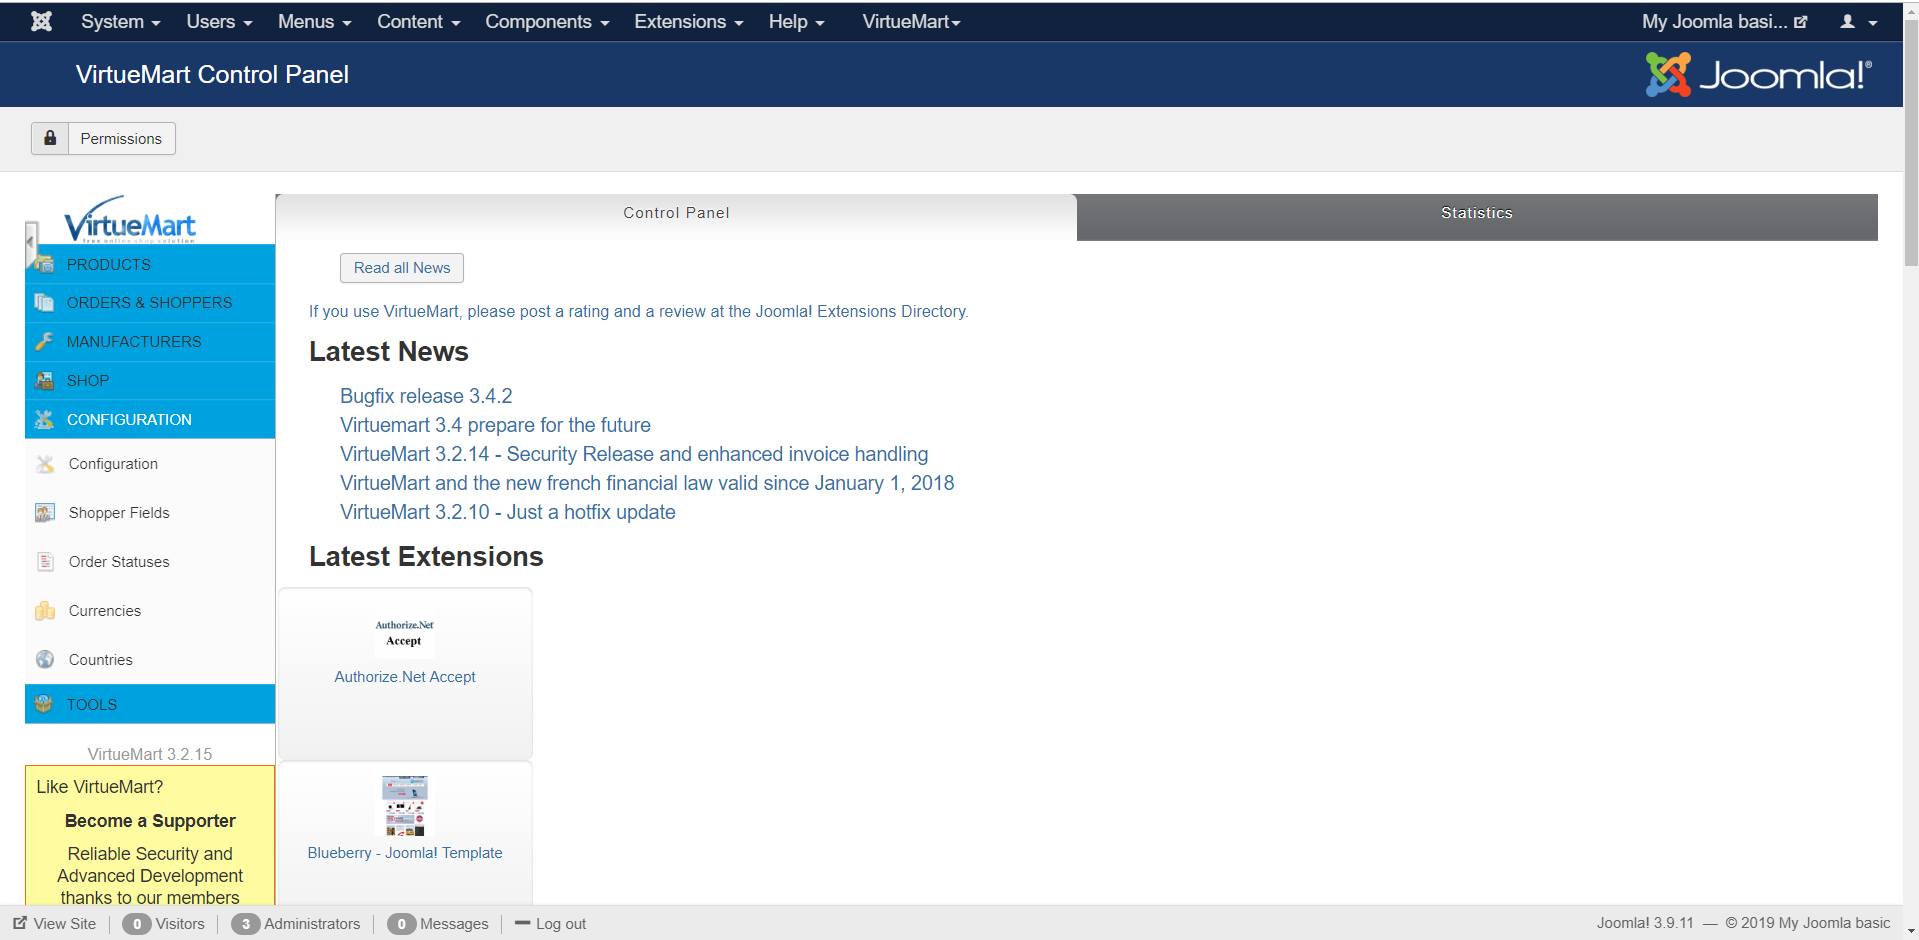
\includegraphics[scale = 0.3]{img/virtuemart_controlpanel.png}
	\caption{De control panel van VirtueMart}
	\label{fig:VMcontrolpanel}
\end{figure}
\subsubsection{Drupal Commerce}
Drupal Commerce is een module dat men installeert op een Drupal omgeving. Dit houdt dus in dat de interface dat we gebruiken om deze te beheren bepaald wordt door Drupal. Voor intuïviteit houdt dit dus in dat deze overeenkomt met de intuïtiviteit van de `backoffice` van Drupal. Als de module succesvol is toegevoegd is er een extra menu item aanwezig in het administratieve menu genaamd Commerce. Hier moet men dus zijn als men het e-commerce gedeelte van de website wil herconfigureren. Het commerce gedeelte is mooi onderverdeeld in enkele subonderdelen met een beschrijving. Dezelfde opmerkingen gelden voor als bij de `backoffice', het voelt niet zo natuurlijk aan als de andere CMS'en tot men er wegwijs geraakt is. Als men de taal geconfigureerd heeft zoals besproken bij de backoffice wordt de taal van het Commerce gedeelte automatisch gelijk gezet. Dit verhoogt de gebruiksvriendelijkheid en helpt om sneller wegwijs te geraken.
\subsection{Support van de e-commerce oplossing}
\subsubsection{WooCommerce}
Indien men support wenst bij WooCommerce moet men deze gaan zoeken op de website. Men zit met een vraag tijdens het gebruiken van WooCommerce. Men kan er voor kiezen om contact op te nemen met WooCommerce. Indien men contact wenst met hun, zijn er drie opties. Men kan het problemen trachtten zelf op te lossen met de documentatie te raadplegen dat zij voorzien hebben. Als men klant is bij hun kan men support aanvragen en indien men geen klant is kan men contact opnemen door het invullen van hun contactformulier. Indien men een complexe custiomazition van WooCommerce kan men via hun terecht voor een langdurige of eenmalige partner. Bij hun documentatie vindt men verschillende types van documentatie terug. Zo is er documentatie aanwezig voor als men juist start met WooCommmerce, maar ook voor het uitbreiden van WooCommerce en ook voor het bouwen \& customize van WooCommerce. Er is ook aparte documentatie aanwezig voor developers.
\subsubsection{VirtueMart}
Indien men meer informatie wenst of meer wilt leren over VirtueMart kan men terecht op de website van VirtueMart. Zo is er een developer portaal aanwezig alsook een documentation portaal. Hier is er ook een forum waar men terecht kan voor specifieke vragen/problemen dat men niet kan oplossen met behulp van de documentatie. Op het documentatie portaal kan men verschillende informatiebronnen terugvinden. Zo zijn er FAQ's aanwezig, waar men veel terugkomende vragen kan terugvinden. Zo zijn er manuals en tutorials aanwezig die u kunnen helpen tijdens het opzetten van een webshop. Men kan er ook meer uitleg vinden over de general concepts van VirtueMart, hier kan men terecht als men meer wilt leren wat er juist allemaal achter VirtueMart zit. Er is ook een technischere bron aanwezig van hun API, deze is bedoeld voor de developers. Het developer portaal is specifieke bedoel voor developers. Hier vindt men de laatste ontwikkeling in de broncode, al de voorgaande versies van VirtueMart, een wiki voor VirtueMart development en de repository met de broncode van VirtueMart.
\subsubsection{Drupal Commerce}
Voor hulp bij het gebruiken van de Drupal Commerce module kan men tercht op hun website. Hier kan men onder andere terecht voor documentatie, video's, betalende support en vroeger Q\&A. De Q\&A bevindt zich niet langer op hun eigen website en is verplaatst naar Drupal Answers, daar kan men nu terecht met vragen over Drupal commerce. Men moet nu de vraag daar stellen onder de tag drupal commerce. Er wordt ook een ruim aanbod van video's aangeboden op hun website gaande van tutorials tot webinars. Men kan ook professionele hulp van hun krijgen gekoppeld aan een toch wat hoog prijskaartje, maar men kan ook altijd een prijsofferte aanvragen voor een specifieke project/website.

Er is natuurlijk ook altijd de documentatie dat men kan raadplegen. Er zijn twee grote vormen van documentatie: de documentatie met als doel om een beter begrip te creëren van Drupal Commerce en de documentatie voor het effectief gebruiken van Drupal Commerce. Bij de eerste vorm is bestaat er een guide voor de developer en de site builder. De developer guide is bedoelt om de workflow, coding standards, achterliggende architectuur, etc. bij te lichten. De guide voor de site builder probeert duidelijkheid te scheppen hoe de verschillende stukken van de module nu juist bij elkaar passen door deze te koppelen aan use cases. Van de tweede vorm bestaan er per versie van Drupal Commerce een User guide en een Developer guide. De user guide helpt bij het gebruiken van de module als eindgebruiker en bij de developer guider logischerwijs voor het gebruiken van de module vanuit het developer standpunt.
\subsection{All-in-one functionaliteit van de e-commerce oplossing}
Hier gaat men kijken wat er standaard al mee wordt aangeboden in de oplossing. Men zal dus kijken over welke standaard functionaliteit men beschikt zonder het installeren van extra modules/plug-ins.
\subsubsection{WooCommerce}
Zoals in het intuïtivieit tijd stuk is aangehaald, zijn er twee nieuwe menu items aanwezig in de main navigatie. Deze items zijn WooCommerce en Producten. Onder het WooCommerce gedeelte is men in staat om bestellingen en kortingsbonnen te beheren. Men kan er een hele reeks aan rapporten raadplegen in verband met verkoop, klanten en voorraad. Men kan er de instellingen beheren, onder deze instellingen vallen volgende zaken: algemene informatie van de winkel, instellingen omtrent producten, verzendmethoden, betalingen, accounts \& privacy, e-mails en geavanceerd(bv. configureren van een REST API key). Hiernaast kan men ook de status van WooCommerce raadplegen en wordt de achterliggende configuratie verzameld van de website. Hier krijgt men dan suggesties om zaken te veranderen waardoor de webshop beter zal werken. Als laatste is er dan nog een overzicht van extensions dat men misschien wilt gebruiken. Onder het producten gedeelte is men logischerwijs in staat om onze producten te beheren en nieuwe producten aan te maken. Men kan hier ook de categorieën, tags en attributen beheren die toegewezen kunnen worden aan producten. Met al deze zaken is men perfect in staat om een werkende webshop op te zetten. Soms zal men deze functionaliteit moeten uitbreiden met behulp van plug-ins.

\subsubsection{VirtueMart}

\subsubsection{Drupal Commerce}
Bij een standaard installatie van Drupal Commerce is er al redelijk wat functionaliteit aanwezig. Zo is er na installatie de cart, checkout, payment, promotion en tax functionaliteit toegevoegd. Hiernaast worden er nog verscheidende entiteiten geïnstalleerd die noodzakelijk zijn voor een werkende e-commerce oplossing. Deze module definieert order, valuta, product en winkel entiteiten en hun bijhorende features. Al de activiteiten dat omtrent het Commerce gedeelte van de website gebeuren worden verzameld in de commerce logs, die dankzij commerce module beschikbaar zijn. 

Na de installatie is men dus in staat om volgende zaken te doen:
\begin{itemize}
	\item Aanmaken van verschillende winkels en verschilende producten
	\item Beheren van de verschillende valuta's dat geacepteerd worden
	\item Belasting innen op de producten dat men aanbiedt
	\item Opzetten van promoties 
	\item Definiëren van verschillende ordertypes
	\item Configuren van de checkout procedure
	\item Configuren van het betalingsportaal
	\item Raadplegen van specifieke commerce logs indien er fouten optreden.
\end{itemize}

Men kan dus concluderen dat er een ruim aanbod aan functionaliteit voorzien is in de standaard installatie van de Drupal Commerce module. Met deze functionaliteit is men perfect in staat om een werkende webshop op te zetten.
\subsection{Governance van de e-commerce oplossing}
\subsubsection{WooCommerce}
WooCommerce is een uitbreiding dat men bovenop Wordpress installeert. Dit houdt dus in dat men de rechten omtrent het beheer van het e-commerce aspect moeten configureren gelijk dit in Wordpress gebeurt. In Wordpress wordt er gebruik gemaakt van roles en capabilites om te bepalen wie welke rechten bezit. In het Governance gedeelte van de algemene vergelijking leerde men al dat Wordpress 6 roles heeft gedefinieerd en dat men enkel nieuwe kan toevoegen door middel van code of een externe plug-in. Tijdens de installatie van Wordpress worden er twee nieuwe roles toegevoegd namelijk de customer rol en de shop manager rol. Een customer heeft enkel leesrechten op de website (zoals de subscriber rol), kan zijn eigen account informatie aanpassen en kan vroegere en huidige bestellingen bekijken. De rechten van de shop manager zijn als volgt: de rechten van de customer rol + algemene Wordpress editor capabilities + volledige managementrechten voor WooCommerce \& producten + toegang tot alle WooCommerce rapporten.
\subsubsection{VirtueMart}

\subsubsection{Drupal Commerce}
Zoals eerder aangehaald bij het intuïtiviteit gedeelte, runt de Drupal Commerce bovenop Drupal. Dit houdt dus in dat de rechten omtrent de Commerce module gelijk de rechten in Drupal bepaald worden. Men zal dus aan de slag moeten gaan met de rollen en permissies om te bepalen wie, wat mag kunnen in de Commerce omgeving. Zoals gewoonlijk heeft een administrator rechten om alles te doen in de commerce module. Voor authenticated en anonymous users gelden er beperkingen. Zo heeft een anonymous user enkel rechten om volgende zaken te doen: afrekenen en producten bekijken. De Authenticated user heeft dezelfde rechten plus twee extra namelijk: Bekijken van zijn bestelling en beheren van zijn betaalopties. Dit zijn natuurlijk de standaard rechten. Natuurlijk kan men deze permissies achteraf nog aanpassen naar wens van de site builder. 

Zo kan men bijvoorbeeld opteren voor de shop manager rol te definiëren. Deze rol zal alle permissies bezitten die vereist zijn om het e-commerce gedeelte van de website te beheren, maar belemmerd zijn in andere rechten. Zo kan de verantwoordelijk van de shop, de nodige aanpassingen doen zonder al te veel schade aan te richten op de rest van de website. Dit alles kan men makkelijk realiseren via de admin interface.
\subsection{SEO van de e-commerce oplossing}
Bij de SEO van een webshop zijn er nog enkele zaken dat een bepalende rol spelen in de SEO-score. Het is belangrijk dat men bij productafbeelding een passend bestaandsnaam en alt-beschrijving voorzien, een unieke productomschrijving, interne links(bijvoorbeeld naar gerelateerde producten), beteknisvolle paginatitels en leesbare URL's.
\subsubsection{WooCommerce}
De permalink functionaliteit van Wordpress kan ook gebruikt worden in het e-commerce aspect. Men kan dus leesbare en mooie URL's definiëren voor de verschillende aspecten van de webshop en voor de producten. De taxonomies die aanwezig zijn in Wordpress kan men ook gebruiken bij de producten. Zo is men in staat om gerelateerde producten met elkaar te verbinden en een vlottere navigatie te voorzien. Bij de algemene info van een product is men in staat om gerelateerde producten effectief te gaan linken aan dit product. Niet met behulp van taxonomie maar het effectief ingeven van de link naar een ander product. Dit zal de navigatie door de website verhogen. Deze aspecten spelen een rol in de SEO-score en kunnen dus helpen om deze te verbeteren.
\subsubsection{VirtueMart}
\subsubsection{Drupal Commerce}
Het voorzien van deze leesbare URL's kan men realiseren door gebruik te maken van de URL-aliassen functionaliteit. De taxonomie zal hier ook van pas komen om de producten van de webshop beter te categoriseren. Deze twee factoren beinvloed de SEO-score op een positieve manier.
